\chapter{Základné pojmy a definície}

\label{kap:definitions} % id kapitoly pre prikaz ref

\textit{Útvar} definujeme ako neprázdnu množinu bodov v konečnej geometrii. \textit{Prvok} je bod útvaru, ktorý má priradenú hodnotu $x$, kde $x$ je kladné celé číslo. Prvky musia mať priradené navzájom rôzne hodnoty. \\

Ľubovoľnú neprázdnu podmnožinu bodov nazývame \textit{skupinou}. Každý útvar má priradený nenulový počet skupín. Hovoríme, že útvar má \textit{magickú vlastnosť}, ak všetky jeho skupiny majú magickú vlastnosť.

\section{Magické útvary}
\begin{definition} Útvar je \textbf{magický}, ak súčty prvkov v jednotlivých skupinách sú rovnaké.
\end{definition}

\subsection{Magické štvorce}
\begin{definition} \textbf{Magický štvorec} je matica prvkov veľkosti $n \times n$, pre ktorú platí, že súčty prvkov v riadkoch, stĺpoch a na oboch diagonálach sú rovnaké \cite{multimagie}.
\end{definition}

\begin{center}
$\begin{array}{ |c|c|c| } 
\hline
4 & 3 & 8 \\ 
\hline
9 & 5 & 1 \\ 
\hline
2 & 7 & 6 \\
\hline
\end{array}$
\end{center}

Skupinami v štvorci sú jeho riadky, stĺpce a diagonály.

\begin{definition} Ak je súčet prvkov v každom riadku a stĺpci rovnaký, daný štvorec nazývame \textbf{semimagickým}.
\end{definition}

\begin{definition} Ak sú prvkami čísla z množiny $\{1, \dots, n^2\}$, daný štvorec nazývame \textbf{supermagickým}.
\end{definition}

Špeciálnu triedu tvoria magické štvorce, ktorých prvky sú $k$-tymi mocninami kladných celých čísel. Príklad štvorca pre $n = 4, k = 2$ \cite{multimagie}:

\begin{center}
$\begin{array}{ |c|c|c|c| } 
\hline
48^2 & 23^2 & 6^2 & 19^2 \\ 
\hline
21^2 & 26^2 & 33^2 & 32^2 \\ 
\hline
1^2 & 36^2 & 13^2 & 42^2 \\
\hline
22^2 & 27^2 & 44^2 & 9^2 \\
\hline
\end{array}$
\end{center}

Existencia štvorca pre $n = 3, k = 2$ je otvoreným problémom. Je dokázané, že ak by taký štvorec existoval, jeho prvky by museli byť väčšie ako $10^{16}$. Nikomu sa nepodarilo nájsť ani taký magický štvorec, ktorého $8$ prvkov sú druhé mocniny prirodzených čísel. Je známe iba jedno základné riešenie so $7$ prvkami, ktoré objavil v roku 1999 Andrew Bremner \cite{multimagie}:

\begin{center}
$\begin{array}{ |c|c|c| } 
\hline
373^2 & 289^2 & 565^2 \\ 
\hline
360721 & 425^2 & 23^2 \\ 
\hline
205^2 & 527^2 & 222121 \\
\hline
\end{array}$
\end{center}

Pre $n = k = 3$ je dokázané, že takýto magický štvorec neexistuje. Existencia štvorcov pre $4 \leq n \leq 6, k = 3$ je otvoreným problémom. Pre $4 \leq n \leq 10, k \geq 4$ sú známe iba semimagické štvorce \cite{multimagie}.

\subsection{Magické obdĺžniky}
\begin{definition} \textbf{Magický obdĺžnik} je matica prvkov veľkosti $m \times n$, pre ktorú platí, že súčty prvkov v riadkoch sú rovnaké a zároveň súčty prvkov v stĺpcoch sú rovnaké.
\end{definition}

\begin{center}
$\begin{array}{ |c|c|c|c| } 
\hline
1 & 7 & 6 & 4 \\ 
\hline
8 & 2 & 3 & 5 \\
\hline
\end{array}$
\end{center}

\begin{definition} Ak sú prvkami čísla z množiny $\{1, \dots, mn\}$, daný obdĺžnik nazývame \textbf{supermagickým} \cite{rectangles}.
\end{definition}

Semimagické štvorce sú špeciálnym prípadom magických obdĺžnikov pre $m = n$. Preto budeme ďalej predpokladať, že $m \neq n$. \\

Nevyžadujeme, aby boli súčty v riadkoch a stĺpcoch rovnaké, pretože z vlastnosti $m \neq n$ vieme ľahko odvodiť, že by museli byť rovné $0$ (čo je spor s tým, že prvky sú navzájom rôzne kladné celé čísla). Z toho vyplýva, že obdĺžnik má dva druhy skupín: jedna je tvorená riadkami a druhá stĺpcami. \\

Slovenský matematik Marián Trenkler skúmal supermagické obdĺžniky \cite{rectangles}:

\begin{theorem} (Trenkler, 1999) Pre všetky kladné celé $n > 2$ vieme zostrojiť supermagický obdĺžnik veľkosti $2 \times (2n - 2)$ aj $n \times n^2$.
\end{theorem}

\begin{theorem} (Trenkler, 1999) Nech $a,b$ sú kladné celé čísla a $n$ je ich súčin, pričom $n > 2$. Potom vieme zostrojiť supermagický obdĺžnik veľkosti $an \times bn$.
\end{theorem}

\begin{theorem} (Trenkler, 1999) Ak vieme zostrojiť supermagické obdĺžniky veľkosti $m \times n$ aj $p \times q$ pre nejaké $m,n,p,q \in \mathbb{N^+}$, potom vieme zostrojiť aj supermagický obdĺžnik veľkosti $mp \times nq$.
\end{theorem}

Keďže obdĺžniková matica nemá diagonály, pri definícii ich neuvažujeme. Z toho vyplýva, že v ľubovoľnom magickom obdĺžniku vieme vymeniť dva riadky alebo stĺpce a magická vlastnosť ostane zachovaná.

\subsection{Magické grafy}
\begin{definition} \textbf{Magický graf} je neorientovaný graf s ohodnotenými hranami, v ktorom platí, že súčty hodnôt hrán incidentných s jednotlivými vrcholmi sú rovnaké. Vrcholy sú považované za prvky útvaru \cite{antimagic}.
\end{definition}

Z toho vyplýva, že skupiny v grafe sú hodnoty incidentných hrán s daným vrcholom. Príklad magického grafu so súčtom 62 \cite{antimagic}:

\tikzset{every picture/.style={line width=0.75pt}} %set default line width to 0.75pt        
\begin{center}
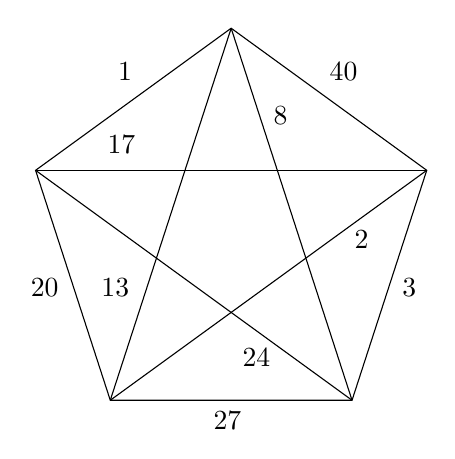
\begin{tikzpicture}[x=0.75pt,y=0.75pt,yscale=-1,xscale=1]
%uncomment if require: \path (0,300); %set diagram left start at 0, and has height of 300

%Shape: Polygon [id:dp4501387538081263] 
\draw   (255.01,202.89) -- (138.53,202.89) -- (102.54,92.11) -- (196.77,23.65) -- (291,92.11) -- cycle ;
%Straight Lines [id:da16990261093603642] 
\draw    (102.54,92.11) -- (291,92.11) ;
%Straight Lines [id:da328363468547485] 
\draw    (138.53,202.89) -- (196.77,23.65) ;
%Straight Lines [id:da1305528921709198] 
\draw    (196.77,23.65) -- (255.01,202.89) ;
%Straight Lines [id:da4209848873821789] 
\draw    (138.53,202.89) -- (291,92.11) ;
%Straight Lines [id:da44373813291222675] 
\draw    (102.54,92.11) -- (255.01,202.89) ;

% Text Node
\draw (141,39) node [anchor=north west][inner sep=0.75pt]   [align=left] {1};
% Text Node
\draw (243,39) node [anchor=north west][inner sep=0.75pt]   [align=left] {40};
% Text Node
\draw (216,60) node [anchor=north west][inner sep=0.75pt]   [align=left] {8};
% Text Node
\draw (99,143) node [anchor=north west][inner sep=0.75pt]   [align=left] {20};
% Text Node
\draw (133,143) node [anchor=north west][inner sep=0.75pt]   [align=left] {13};
% Text Node
\draw (201,177) node [anchor=north west][inner sep=0.75pt]   [align=left] {24};
% Text Node
\draw (255,120) node [anchor=north west][inner sep=0.75pt]   [align=left] {2};
% Text Node
\draw (278,143) node [anchor=north west][inner sep=0.75pt]   [align=left] {3};
% Text Node
\draw (136,74) node [anchor=north west][inner sep=0.75pt]   [align=left] {17};
% Text Node
\draw (187,207) node [anchor=north west][inner sep=0.75pt]   [align=left] {27};
\end{tikzpicture}
\end{center}

Je zrejmé, že kompletné bipartitné regulárne grafy sú ekvivalentné magickým štvorcom. \\

Slovenskí matematici Samuel Jezný a Marián Trenkler dokázali vetu, ktorá hovorí o tom, kedy je graf magický \cite{graphs}:

\begin{theorem} (Jezný, Trenkler, 1983) Graf je magický práve vtedy, keď každá hrana $G$ patrí do nejakého $(1-2)$-faktora a zároveň každá dvojica hrán $e_1, e_2$ je separovateľná $(1-2)$-faktorom grafu $G$.
\end{theorem}

\begin{note} $(1-2)$-faktor grafu je podgraf, ktorý obsahuje všetky vrcholy a zároveň každý jeho komponent je kružnica alebo izolovaná hrana. 
\end{note} 

Magická vlastnosť grafu sa dá skúmať viacerými spôsobmi. Môžeme napríklad pre každý vrchol zrátať súčet hodnôt jeho susedov (v takom prípade budú v skupine hodnoty susedov daného vrchola). V čase písania tejto práce nie sú známe žiadne štúdie, ktoré by sa zaoberali skúmaním bimagických a multiplikatívnych magických vlastností na grafoch. Bimagické a multiplikatívne magické útvary definujeme nižšie.

\section{Multiplikatívne útvary}
\begin{definition} Útvar je \textbf{multiplikatívny}, ak súčiny prvkov v jednotlivých skupinách sú rovnaké \cite{multimagie}.
\end{definition}

\begin{definition} \textbf{Multiplikatívny štvorec} je matica prvkov veľkosti $n \times n$, pre ktorú platí, že súčiny prvkov v riadkoch, stĺpcoch a na oboch diagonálach sú rovnaké.
\end{definition}

\begin{center}
$\begin{array}{ |c|c|c| } 
\hline
8 & 256 & 2 \\ 
\hline
4 & 16 & 64 \\ 
\hline
128 & 1 & 32 \\
\hline
\end{array}$
\end{center}

\begin{note} \textbf{Semimultiplikatívne} štvorce sú definované analogicky.
\end{note}

K ľubovoľnému magickému štvorcu vieme zostrojiť multiplikatívny štvorec napríklad tak, že všetky jeho prvky $x$ nahradíme $2^x$.

\section{Bimagické útvary}
\begin{definition} Útvar je \textbf{bimagický}, ak je magický a umocnením každého jeho prvku na druhú dostaneme opäť magický útvar \cite{multimagie}.
\end{definition}

\begin{note} \textbf{Semibimagické} a \textbf{superbimagické} štvorce sú definované analogicky.
\end{note}

Je zrejmé, že bimagický štvorec veľkosti $2 \times 2$ neexistuje. Edouard Lucas, Luke Pebody a Jean-Claude Rosa dokázali silnejšie tvrdenia \cite{multimagie}:

\begin{theorem} (Lucas, 1891) Neexistuje bimagický štvorec veľkosti $3 \times 3$.
\end{theorem}

\begin{theorem} (Pebody, Rosa, 2004) Neexistuje bimagický štvorec veľkosti $4 \times 4$.
\end{theorem}

Sú známe semibimagické štvorce veľkosti $n \times n$ pre $n \geq 4$. \\

Na to, aby bol štvorec veľkosti $5 \times 5$ bimagickým, muselo by byť jeho 12 magických a 12 bimagických súčtov rovnakých. Čiastočné riešenie našiel Michael Quist v júni 2010. Toto obsahovalo 23 správnych súčtov \cite{multimagie}:

\begin{center}
$\begin{array}{ |c|c|c|c|c| }
\hline
25 & 129 & 200 & 295 & 195 \\ 
\hline
257 & 165 & 1 & 225 & 196  \\ 
\hline
127 & 340 & 171 & 111 & 95 \\ 
\hline
267 & 85 & 265 & 176 & 51 \\ 
\hline
168 & 125 & 207 & 37 & 307 \\
\hline
\end{array}$
\end{center}

Dodnes zostáva otvoreným problémom existencia riešenia pre $5 \times 5$, ktoré by malo 24 správnych súčtov. \\

V roku 2006 našiel Jaroslaw Wroblewski riešenie pre $6 \times 6$ \cite{multimagie}:

\begin{center}
$\begin{array}{ |c|c|c|c|c|c| } 
\hline
17 & 36 & 55 & 124 & 62 & 114 \\ 
\hline
58 & 40 & 129 & 50 & 111 & 20 \\ 
\hline
108 & 135 & 34 & 44 & 38 & 49 \\
\hline
87 & 98 & 92 & 102 & 1 & 28 \\
\hline
116 & 25 & 86 & 7 & 96 & 78 \\
\hline
22 & 74 & 12 & 81 & 100 & 119 \\
\hline
\end{array}$
\end{center}

Georges Pfeffermann objavil v roku 1890 superbimagický štvorec veľkosti $8 \times 8$. Použil v ňom všetky čísla z množiny $\{1, 2, \dots , 64\}$ \cite{multimagie}:

\begin{center}
$\begin{array}{ |c|c|c|c|c|c|c|c| }
\hline
56 & 34 & 8 & 57 & 18 & 47 & 9 & 31 \\ 
\hline
33 & 20 & 54 & 48 & 7 & 29 & 59 & 10 \\ 
\hline
26 & 43 & 13 & 23 & 64 & 38 & 4 & 49 \\ 
\hline
19 & 5 & 35 & 30 & 53 & 12 & 46 & 60 \\ 
\hline
15 & 25 & 63 & 2 & 41 & 24 & 50 & 40 \\ 
\hline
6 & 55 & 17 & 11 & 36 & 58 & 32 & 45 \\ 
\hline
61 & 16 & 42 & 52 & 27 & 1 & 39 & 22 \\ 
\hline
44 & 62 & 28 & 37 & 14 & 51 & 21 & 3 \\ 
\hline
\end{array}$
\end{center}

Nasledovná veta dokazuje, že bimagických štvorcov je nekonečne veľa \cite{bimagic}:

\begin{theorem} (Chen, Li, 2004) Nech $m,n$ sú kladné celé čísla s rovnakou paritou, pričom $m,n \notin \{2,3,6\}$. Potom existuje superbimagický štvorec veľkosti $mn \times mn$.
\end{theorem}

\section{Multiplikatívne magické útvary}
\begin{definition} Útvar je \textbf{multiplikatívny magický}, ak je magický aj multiplikatívny~\cite{multimagie}.
\end{definition}

Je zrejmé, že multiplikatívny magický štvorec veľkosti $2 \times 2$ neexistuje. Lee Morgenstern dokázal silnejšie tvrdenie \cite{multimagie}:

\begin{theorem} (Morgenstern, 2007) Neexistuje multiplikatívny magický štvorec veľkosti $3 \times 3$ ani $4 \times 4$.
\end{theorem}

Morgenstern taktiež skúmal multiplikatívne magické štvorce veľkosti $5 \times 5$ a $6 \times 6$. V roku 2007 našiel nasledovný štvorec s jedinou skupinou, ktorá nemá multiplikatívnu magickú vlastnosť \cite{multimagie}:

\begin{center}
$\begin{array}{ |c|c|c|c|c| }
\hline
105 & 182 & 40 & 198 & 45 \\ 
\hline
78 & 216 & 66 & 175 & 35  \\ 
\hline
220 & 42 & 65 & 63 & 180 \\ 
\hline
140 & 55 & 189 & 30 & 156 \\ 
\hline
27 & 75 & 210 & 104 & 154 \\ 
\hline
\end{array}$
\end{center}

Objavil aj tento semimultiplikatívny magický štvorec (nemá multiplikatívne diagonály) \cite{multimagie}:

\begin{center}
$\begin{array}{ |c|c|c|c|c|c| }
\hline
27 & 25 & 156 & 48 & 84 & 20 \\ 
\hline
75 & 144 & 18 & 56 & 52 & 15 \\ 
\hline
24 & 12 & 45 & 117 & 50 & 112 \\ 
\hline
16 & 65 & 21 & 30 & 108 & 120 \\ 
\hline
140 & 72 & 40 & 9 & 60 & 39 \\ 
\hline
78 & 42 & 80 & 100 & 6 & 54 \\
\hline
\end{array}$
\end{center}

V roku 2016 našiel Sébastien Miquel riešenie pre veľkosť $7 \times 7$  \cite{multimagie}:

\begin{center}
$\begin{array}{ |c|c|c|c|c|c|c| } 
\hline
126 & 66 & 50 & 90 & 48 & 1 & 84 \\ 
\hline
20 & 70 & 16 & 54 & 189 & 110 & 6 \\ 
\hline
100 & 2 & 22 & 98 & 36 & 72 & 135 \\
\hline
96 & 60 & 81 & 4 & 10 & 49 & 165 \\
\hline
3 & 63 & 30 & 176 & 120 & 45 & 28 \\
\hline
99 & 180 & 14 & 25 & 7 & 108 & 32 \\
\hline
21 & 24 & 252 & 18 & 55 & 80 & 15 \\
\hline
\end{array}$
\end{center}

Existencia multiplikatívneho magického štvorca veľkosti $5 \times 5$ alebo $6 \times 6$ zostáva naďalej otvoreným problémom.











